\documentclass[11pt]{article}
\usepackage[margin=1.15in]{geometry}
\usepackage[T1]{fontenc}
\usepackage{lmodern}
\usepackage{amsmath,amssymb,amsthm,mathtools}
\usepackage{microtype}
\usepackage{graphicx}
\usepackage{booktabs}
\usepackage{enumitem}
\usepackage[colorlinks=true,linkcolor=black,citecolor=black,urlcolor=black]{hyperref}

\newtheorem{maintheorem}{Theorem}
\renewcommand{\themaintheorem}{\Alph{maintheorem}}
\newtheorem{theorem}{Theorem}[section]
\newtheorem{proposition}[theorem]{Proposition}
\newtheorem{lemma}[theorem]{Lemma}
\theoremstyle{definition}
\newtheorem{definition}[theorem]{Definition}
\newtheorem{example}[theorem]{Example}
\theoremstyle{remark}
\newtheorem{remark}[theorem]{Remark}
\numberwithin{equation}{section}

\newcommand{\R}{\mathbb{R}}
\newcommand{\E}{\mathbb{E}}
\newcommand{\cL}{\mathcal{L}}
\newcommand{\cK}{\mathcal{K}}
\newcommand{\cB}{\mathcal{B}}
\newcommand{\cR}{\mathcal{R}}
\newcommand{\cT}{\mathcal{T}}
\newcommand{\cP}{\mathcal{P}}
\newcommand{\eps}{\varepsilon}
\newcommand{\sm}{\setminus}
\newcommand{\ip}[2]{\langle #1,#2\rangle}
\newcommand{\id}{\mathrm{id}}
\newcommand{\Sym}{\operatorname{sym}}
\newcommand{\ND}[1]{\textup{(ND#1)}}

\title{Saddle-to-saddle dynamics of deep polynomial ResNets}
\author{}
\date{November 2026}

\begin{document}
\maketitle

\begin{abstract}
We consider gradient flow on residual networks $(\id+\sigma\circ A_L)\circ\dots\circ(\id+\sigma\circ A_1)$ of arbitrary depth $L$ and width $d$, where the $A_j$ are affine maps and the activation $\sigma$ is a polynomial vanishing to order $k\ge3$ at the origin, e.g.\ $\sigma(z)=z^k$. We prove that, as the scale $\alpha$ of the initialization tends to zero and time is rescaled by $\alpha^{2-k}$, the trajectory converges to a jump process. The process rests at critical points of the loss lying in subspaces where the incoming weights of all inactive neurons vanish, and it jumps between these subspaces along explicit escape orbits, each jump activating exactly one neuron. During a plateau, the rescaled weights of each inactive neuron follow the gradient flow of its utility, and a neuron activates when its rescaled weights blow up. The result holds under explicit non-degeneracy conditions. For Gaussian initializations, these reduce almost surely to a condition on the data alone.
\end{abstract}

\section{Introduction}

Trained by gradient flow from a small initialization, many neural networks learn in stages: long plateaus, during which the loss barely moves, alternate with sudden drops. The expected explanation is a \emph{saddle-to-saddle} dynamics. Near the origin, neurons are inactive and the loss is flat in their directions. During a plateau, the inactive neurons stay small but align with useful directions, until one of them escapes and the trajectory moves to a new saddle, where the active neurons form a larger subnetwork. In the limit of vanishing initialization, with time rescaled by the escape time, the trajectory should degenerate into a jump process between saddles. This limit has been proved for diagonal linear networks~\cite{PF23}, where it is also derived from the alternating gradient flows of~\cite{KMC25}, and for two-layer ReLU networks on orthogonal data~\cite{TBLEL26}. For deep networks, the escape from the origin and the dynamics up to the next saddle have been analysed~\cite{JGSHG21,KH24,KH24b,KH25,BSJ25}, but the full limit has remained conjectural.

This note proves the limit for deep residual networks with polynomial activation $\sigma$ vanishing to order $k\ge3$ at the origin (Theorem~\ref{thm:main}). It holds for every depth $L$ and width $d$, with or without biases, and for every smooth loss. In the time scale $s=\alpha^{k-2}t$, the trajectory from $\alpha\xi$ converges to a process that rests at points $\theta^{(m)}$. Each $\theta^{(m)}$ is a critical point of the loss in the subspace $S_{A_m}$ where the incoming weights of the neurons outside a set $A_m$ vanish. The process jumps from $S_{A_m}$ to $S_{A_{m+1}}$, with $A_{m+1}=A_m\cup\{n_{m+1}\}$, along an explicit heteroclinic orbit. The process is explicit: inactive neurons are frozen at scale $\alpha$, and their rescaled weights follow the gradient flow of their \emph{utility}. A neuron activates when its rescaled weights blow up, equivalently when the utility it has accumulated reaches a threshold set by its initialization (Remark~\ref{rem:interpretation}). The active subnetwork then instantly descends to a local minimum of its own loss. The theorem assumes non-degeneracy conditions along the process. For Gaussian initializations, those that depend on the initialization hold almost surely (Theorem~\ref{thm:gaussian}), leaving a condition on the data alone.

Two structural features of these ResNets drive the proof. First, every parameter is an incoming weight of some neuron, because the skip connections play the role of outgoing weights. Second, the incoming weights $w_n$ of a neuron enter the network only through $\sigma(\ip{w_n}{\hat h})$, where $\hat h$ is the input of its layer. Hence the loss is flat of order $k$ along every hyperplane $\{w_n=0\}$, whatever the depth (Proposition~\ref{prop:structure}). The rest is a local analysis near the saddles, in which depth enters only through the utilities and the restricted losses. The central step is the escape from a saddle (Lemma~\ref{lem:escape}). It is degenerate, since the escaping direction has zero linearization. We handle it with the radial time $\log|w_n|$, in which the dynamics becomes a contraction. The assumption $k\ge3$ matters: for $k=2$, deep ResNets have a degeneracy at the origin that makes the first jump depend on the initialization in a more singular way (Remark~\ref{rem:k2}).

Section~\ref{sec:setting} states the results, Sections~\ref{sec:flatness}--\ref{sec:proof-gaussian} contain the proofs, and Section~\ref{sec:numerics} compares the theorem with simulations.

\section{Setting and main results}\label{sec:setting}

\subsection{Deep ResNets}

Fix a width $d\ge1$, a depth $L\ge1$, and a polynomial activation $\sigma\colon\R\to\R$. Let $k\ge2$ be the order of vanishing of $\sigma$ at the origin,
\begin{equation}\label{eq:order}
\sigma(0)=\sigma'(0)=\dots=\sigma^{(k-1)}(0)=0\neq\sigma^{(k)}(0),
\end{equation}
so that $0$ is a critical point of $\sigma$ of order $k$ with critical value $0$; for instance, $\sigma(z)=z^k$. Our main results assume $k\ge3$. The ResNet of depth $L$ and width $d$ is
\begin{equation}\label{eq:resnet}
h_0(x)=x,\qquad h_j(x)=h_{j-1}(x)+\sigma\big(W_jh_{j-1}(x)+b_j\big)\quad(1\le j\le L),\qquad f_\theta(x)=h_L(x),
\end{equation}
where $\theta=(W_1,b_1,\dots,W_L,b_L)$, $W_j\in\R^{d\times d}$, $b_j\in\R^d$, and $\sigma$ acts coordinate-wise. In other words, $f_\theta=(\id+f^{(L)})\circ\dots\circ(\id+f^{(1)})$ with $f^{(j)}(x)=\sigma(W_jx+b_j)$. This is a multilayer perceptron with all widths equal to $d$ and a skip connection at every layer. Everything below holds verbatim without biases (Remark~\ref{rem:variants}).

If $r=\deg\sigma$, then $f_\theta$ is a polynomial map $\R^d\to\R^d$ of degree at most $r^L$, whose coefficients are polynomials in $\theta$. Let $V$ be the finite-dimensional space of polynomial maps $\R^d\to\R^d$ of degree at most $r^L$, and let $\varphi\colon\Theta\to V$, $\theta\mapsto f_\theta$, be the parametrization. We fix a loss $\cL\colon V\to\R$ of class $C^\infty$ and set
\[
F:=\cL\circ\varphi\colon\Theta\to\R .
\]
(The letter $L$ denotes the depth throughout.) The main example is the mean squared error $\cL(f)=\frac12\E\|f(x)-y\|^2$. The expectation is over a finite dataset, or over a probability distribution of $(x,y)$ with $\E\|x\|^{2r^L}<\infty$ and $\E\|y\|^2<\infty$; in both cases $F$ is a polynomial. We study the gradient flow $\dot\theta=-\nabla F(\theta)$ for the Euclidean scalar product on $\Theta$, started at small initializations $\theta(0)=\alpha\xi$, with $\xi\in\Theta$ fixed and $\alpha>0$. We write $\theta^\alpha$ for the maximal solution.

\subsection{Neurons, inactive subspaces, utilities}

A \emph{neuron} is a pair $n=(j,i)$ with $1\le j\le L$ and $1\le i\le d$, namely the $i$-th coordinate of layer $j$. There are $N=Ld$ of them. The \emph{incoming weights} of $n$ are
\[
w_n:=\big(W_j[i,:],\,b_j[i]\big)\in\R^p,\qquad p:=d+1 .
\]
With $\hat h:=(h,1)\in\R^p$, the pre-activation of $n$ is $\ip{w_n}{\hat h_{j-1}(x)}$, and $h_j(x)_i=h_{j-1}(x)_i+\sigma(\ip{w_n}{\hat h_{j-1}(x)})$. Thus $\Theta=(\R^p)^N$ and $\theta=(w_n)_n$. The network has no other parameters. For a set $A$ of neurons, the \emph{active} ones, let
\[
S_A:=\{\theta\in\Theta:\ w_n=0\text{ for all }n\notin A\}.
\]
On $S_A$, the neurons outside $A$ are inactive: their pre-activation and output vanish identically. Let $\pi_A$ be the orthogonal projection onto $S_A$, $F_A:=F|_{S_A}$, and $\theta^{\sm n}:=\pi_{[N]\sm\{n\}}\theta$, i.e., $\theta$ with $w_n$ replaced by $0$. For $w\in\R^p$, $\iota_n(w)\in\Theta$ is the parameter whose $n$-th component is $w$ and whose other components vanish. For a trajectory $\gamma$ in $\Theta$, $\gamma_n$ denotes its $n$-th component.

\begin{definition}[Utility]
For $\theta\in\Theta$ and a neuron $n$, the \emph{utility} of $n$ at $\theta$ is the homogeneous polynomial of degree $k$
\[
U_n(\theta;w):=-\frac1{k!}\,\frac{d^k}{d\tau^k}\Big|_{\tau=0}F\big(\theta^{\sm n}+\tau\,\iota_n(w)\big),\qquad w\in\R^p .
\]
It depends on $\theta$ only through $\theta^{\sm n}$.
\end{definition}

\begin{proposition}[Structure of the loss]\label{prop:structure}
The following hold for every depth $L$ and width $d$.
\begin{enumerate}[label=\textup{(\alph*)}]
\item\emph{(Flatness.)} For every neuron $n$, all partial derivatives of $F$ of orders $1,\dots,k-1$ with respect to the coordinates of $w_n$ vanish on the hyperplane $\{w_n=0\}$.
\item\emph{(Invariant subspaces.)} Every $S_A$ is invariant under the gradient flow of $F$, on which it coincides with the gradient flow of $F_A$. In particular, the critical points of $F_A$ are critical points of $F$.
\item\emph{(Utilities.)} If $w_n=0$, then $F(\theta+\iota_n(w))=F(\theta)-U_n(\theta;w)+O(|w|^{k+1})$ as $w\to0$. For the mean squared error and $n=(j,i)$,
\begin{equation}\label{eq:utility}
U_n(\theta;w)=c_\sigma\,\E\Big[\ip{w}{\hat h_{j-1}(x)}^k\,\big(D\Phi_j(h_j(x))^{\top}(y-f_\theta(x))\big)_i\Big],\qquad c_\sigma:=\frac{\sigma^{(k)}(0)}{k!},
\end{equation}
where $\Phi_j:=(\id+f^{(L)})\circ\dots\circ(\id+f^{(j+1)})$ is the map computed by the layers after $j$, so that $f_\theta=\Phi_j\circ h_j$, and all quantities are computed at $\theta$. In particular, $U_{(j,i)}(0;w)=c_\sigma\E[\ip{w}{\hat x}^k(y_i-x_i)]$ for every layer $j$.
\item\emph{(Saddles.)} Let $\theta\in S_A$ be a critical point of $F_A$. If $U_n(\theta;w)>0$ for some $n\notin A$ and $w\in\R^p$, then $\theta$ is a saddle point of $F$: a critical point which is not a local minimum.
\end{enumerate}
\end{proposition}

By \eqref{eq:utility}, the utility of an inactive neuron is the correlation between the $k$-th power of its would-be pre-activation and the residual back-propagated to its output coordinate. By (c), it is the leading-order decrease of the loss when the neuron is switched on along $w$. The last formula in (c) shows a degeneracy due to depth: at $\theta=0$, the $L$ neurons $(1,i),\dots,(L,i)$ of each column $i$ have the same utility.

\subsection{Escape orbits}

A \emph{non-degenerate local minimum} of $F_A$ is a point $\theta^*\in S_A$ with $\nabla F_A(\theta^*)=0$ and $\nabla^2F_A(\theta^*)$ positive definite; for $A=\emptyset$, $S_\emptyset=\{0\}$ and $\theta^*=0$ is one. For $k\ge3$, every active neuron $n\in A$ has $w_n\neq0$ at such a point, since by Proposition~\ref{prop:structure}(a) the Hessian of $F_A$ vanishes in the directions of $w_n$ wherever $w_n=0$. A \emph{non-degenerate local maximum} of a smooth function on the sphere $S^{p-1}$ is a critical point at which its Riemannian Hessian is negative definite. For a homogeneous polynomial $U$ and a critical point $u$ of $U|_{S^{p-1}}$, this Hessian is the restriction of $\nabla^2U(u)-\ip{\nabla U(u)}{u}I$ to $u^\perp$.

\begin{proposition}[Escape orbits]\label{prop:escape}
Let $k\ge3$, let $\theta^*$ be a non-degenerate local minimum of $F_A$, let $n\notin A$, and let $u^*\in S^{p-1}$ be a non-degenerate local maximum of the restriction of $U:=U_n(\theta^*;\cdot)$ to $S^{p-1}$, with $U(u^*)>0$. Then there is a solution $\gamma\colon(-\infty,0]\to\Theta$ of the gradient flow, with values in $S_{A\cup\{n\}}$, such that
\[
\gamma(t)\to\theta^*\quad\text{and}\quad \frac{\gamma_n(t)}{|\gamma_n(t)|}\to u^*\qquad\text{as }t\to-\infty,
\]
and it is unique up to translation in time. Its maximal extension is the \emph{escape orbit} of $\theta^*$ along $(n,u^*)$.
\end{proposition}

This is proved in Lemma~\ref{lem:escape}(a). The orbit $\gamma$ plays the role of an unstable manifold, but the saddle is degenerate: in the time $t$, the coordinates of $w_n$ have zero linearization. In the radial time $\log|w_n|$, the direction $w_n/|w_n|$ is attracted to $u^*$, the active coordinates are attracted even faster, and the radius grows; the proof is a contraction argument in this time. Numerically, $\gamma$ is approximated by the gradient flow of $F_{A\cup\{n\}}$ started at $\theta^*+\iota_n(\eps u^*)$ for small $\eps>0$, by Lemma~\ref{lem:escape}(b).

\subsection{The limit process}

\begin{definition}[Saddle-to-saddle process]\label{def:process}
Let $k\ge3$ and $\xi\in\Theta$. We define recursively times $0=s_0<s_1<\dots$, active sets $\emptyset=A_0\subsetneq A_1\subsetneq\dots$, points $\theta^{(m)}\in S_{A_m}$, and dormant curves $\Xi_n$.
\begin{itemize}
\item \emph{Stage $0$.} $s_0=0$, $A_0=\emptyset$, $\theta^{(0)}=0$, and $\Xi_n(0)=\xi_n$ for every neuron $n$.
\item \emph{Stage $m$.} Suppose that $s_m$, $A_m$, a non-degenerate local minimum $\theta^{(m)}$ of $F_{A_m}$, and $\Xi_n(s_m)$ for $n\notin A_m$ are given. Let $U_n^{(m)}:=U_n(\theta^{(m)};\cdot)$. For $n\notin A_m$, let $\Xi_n\colon[s_m,s_m+T_n^{(m)})\to\R^p$, with $T_n^{(m)}\in(0,\infty]$, be the maximal solution of
\begin{equation}\label{eq:dormant}
\frac{d}{ds}\Xi_n(s)=\nabla U_n^{(m)}\big(\Xi_n(s)\big)
\end{equation}
with the given initial value at $s_m$, and let $s_{m+1}:=s_m+\min_{n\notin A_m}T_n^{(m)}$. If $s_{m+1}=\infty$, the construction stops. Otherwise, stage $m$ is \emph{non-degenerate} if:
\begin{enumerate}[label=\textup{(ND\arabic*)},leftmargin=4em]
\item the minimum is attained at a single neuron $n_{m+1}$;
\item as $s\uparrow s_{m+1}$, the direction $\Xi_{n_{m+1}}(s)/|\Xi_{n_{m+1}}(s)|$ converges to a non-degenerate local maximum $u_{m+1}$ of $U^{(m)}_{n_{m+1}}|_{S^{p-1}}$;
\item the escape orbit $\gamma_{m+1}$ of $\theta^{(m)}$ along $(n_{m+1},u_{m+1})$ is defined for all $t\ge0$ and converges, as $t\to\infty$, to a non-degenerate local minimum $\theta^{(m+1)}$ of $F_{A_{m+1}}$, where $A_{m+1}:=A_m\cup\{n_{m+1}\}$.
\end{enumerate}
In that case, set $\Xi_n(s_{m+1}):=\lim_{s\uparrow s_{m+1}}\Xi_n(s)$ for $n\notin A_{m+1}$, which exists since $T^{(m)}_n>s_{m+1}-s_m$, and pass to stage $m+1$. If stage $m$ is degenerate, the construction stops.
\end{itemize}
Let $M$ be the last stage reached, so that either $s_{M+1}=\infty$ or stage $M$ is degenerate. The \emph{limit path} is $\bar\theta(s):=\theta^{(m)}$ for $s_m\le s<s_{m+1}$ and $m\le M$. Each $\Xi_n$ is defined and continuous on $[0,\bar s_n)$, where $\bar s_n:=s_m$ if $n=n_m$, and $\bar s_n:=s_M+T^{(M)}_n\ge s_{M+1}$ if $n\notin A_M$.
\end{definition}

In \ND2, Proposition~\ref{prop:escape} applies because $U^{(m)}_{n_{m+1}}(u_{m+1})>0$ automatically (Remark~\ref{rem:interpretation}). Since every jump activates a new neuron, there are at most $N$ jumps.

\begin{remark}[Interpretation]\label{rem:interpretation}
Write a dormant state as $\Xi_n=R_nu_n$ with $R_n=|\Xi_n|$ and $|u_n|=1$, and let $U=U^{(m)}_n$. By Euler's identity $\ip{u}{\nabla U(u)}=kU(u)$, equation \eqref{eq:dormant} reads
\[
\frac{d}{ds}R_n^{2-k}=-k(k-2)\,U(u_n),\qquad \frac{d}{ds}u_n=R_n^{k-2}\,\nabla_{S}U(u_n),
\]
where $\nabla_S$ is the spherical gradient. Hence
\[
R_n(s)^{2-k}=|\xi_n|^{2-k}-k(k-2)\int_0^sU_n^{(m(s'))}\big(u_n(s')\big)\,ds',
\]
where $m(s')$ is the stage containing $s'$. Neuron $n$ activates when the utility accumulated along its direction reaches $|\xi_n|^{2-k}/(k(k-2))$. Meanwhile, its direction performs gradient ascent of its utility on the sphere, at speed $R_n^{k-2}$, aligning with the directions along which its activation would decrease the loss the most. When a neuron activates, the active subnetwork instantly follows the escape orbit and descends to a local minimum of its own loss, where it remains during the next plateau. This is the alternation of utility maximization and cost minimization of~\cite{KMC25}, here as the exact limit of gradient flow. In the time $\tau$ defined by $d\tau=R_n^{k-2}ds$, the direction $u_n$ follows the gradient flow of $U|_{S^{p-1}}$ and $\frac{d}{d\tau}\log R_n=kU(u_n)$, where $U(u_n(\tau))$ is non-decreasing. Hence a blow-up forces $\tau\to\infty$ and $U(u_n(\tau))\to c>0$. By {\L}ojasiewicz's theorem~\cite{Loj84}, $u_n$ then converges to a critical point $u$ of $U|_{S^{p-1}}$ with $U(u)=c>0$. \ND2 asks that $u$ be a non-degenerate local maximum. If $U|_{S^{p-1}}$ is a Morse function, this holds for almost every initial condition (Lemma~\ref{lem:null}).
\end{remark}

\subsection{Main results}

\begin{maintheorem}\label{thm:main}
Let $k\ge3$. Let $L,d\ge1$ be arbitrary, with or without biases, and let $\cL$ be any $C^\infty$ loss. Let $\xi\in\Theta$, and let $M\ge0$ be such that stages $0,\dots,M-1$ of the saddle-to-saddle process are non-degenerate, so that $s_M<\infty$. Let $S\in(s_M,s_{M+1})$. Then, for $\alpha$ small enough, $\theta^\alpha$ is defined on $[0,\alpha^{2-k}S]$, and as $\alpha\to0$:
\begin{enumerate}[label=\textup{(\roman*)}]
\item\emph{(Plateaus.)} For every $\delta>0$, $\theta^\alpha(\alpha^{2-k}s)\to\bar\theta(s)$ uniformly over $s\in[0,S]\sm\bigcup_{m=1}^M(s_m-\delta,s_m+\delta)$. Consequently $F(\theta^\alpha(\alpha^{2-k}s))\to F(\bar\theta(s))$ uniformly on the same set, and $F(\theta^{(0)})>F(\theta^{(1)})>\dots>F(\theta^{(M)})$.
\item\emph{(Dormant neurons.)} For every neuron $n$ and every $\delta>0$, $\alpha^{-1}w_n^\alpha(\alpha^{2-k}s)\to\Xi_n(s)$ uniformly over $s\in[0,\min(S,\bar s_n-\delta)]$.
\item\emph{(Jumps.)} For each $1\le m\le M$ there are times $t^\alpha_m$ with $\alpha^{k-2}t^\alpha_m\to s_m$ such that $\theta^\alpha(t^\alpha_m+t)\to\gamma_m(t)$ uniformly over $t$ in compact subsets of $\R$, for a suitable time translate of $\gamma_m$. Moreover, for every $\delta>0$ smaller than half the gaps between consecutive points of $\{0,s_1,\dots,s_M,S\}$, the curve $\{\theta^\alpha(\alpha^{2-k}s):|s-s_m|\le\delta\}$ converges in Hausdorff distance to the closure $\gamma_m(\R)\cup\{\theta^{(m-1)},\theta^{(m)}\}$ of the escape orbit.
\end{enumerate}
Finally, every $\theta^{(m)}$ is a critical point of $F$, and for $m<M$ it is a saddle point.
\end{maintheorem}

Thus, in the time scale $s=\alpha^{k-2}t$, the trajectory degenerates into plateaus at the saddles $\theta^{(m)}\in S_{A_m}$, separated by instantaneous jumps from $S_{A_{m-1}}$ to $S_{A_m}$ along the escape orbits, and the loss curve becomes a step function (Figure~\ref{fig:loss}).

To state the result for random initializations, let $\cK$ be the smallest set of pairs $(A,\theta)$ with the following properties. First, $(\emptyset,0)\in\cK$. Second, suppose that $(A,\theta)\in\cK$, $n\notin A$, and $u$ is a non-degenerate local maximum of $U_n(\theta;\cdot)|_{S^{p-1}}$ with $U_n(\theta;u)>0$. If the escape orbit of $\theta$ along $(n,u)$ converges to a non-degenerate local minimum $\theta'$ of $F_{A\cup\{n\}}$, then $(A\cup\{n\},\theta')\in\cK$. By construction, $\theta$ is a non-degenerate local minimum of $F_A$ for every $(A,\theta)\in\cK$. The configurations in $\cK$ depend on the data, but not on $\xi$. We say that \emph{condition \textup{(G)}} holds if, for every $(A,\theta)\in\cK$:
\begin{enumerate}[label=\textup{(G\arabic*)},leftmargin=4em]
\item for every $n\notin A$ and every non-degenerate local maximum $u$ of $U_n(\theta;\cdot)|_{S^{p-1}}$ with $U_n(\theta;u)>0$, the escape orbit of $\theta$ along $(n,u)$ is defined for all $t\ge0$ and converges to a non-degenerate local minimum of $F_{A\cup\{n\}}$;
\item for every $n\notin A$, the restriction of $U_n(\theta;\cdot)$ to $S^{p-1}$ is a Morse function or vanishes identically.
\end{enumerate}
Under (G2), each configuration has finitely many successors, so $\cK$ is finite.

\begin{maintheorem}\label{thm:gaussian}
Let $k\ge3$ and assume \textup{(G)}. Let $\xi$ be a random vector in $\Theta$ whose law has a density, e.g.\ $\xi\sim N(0,I)$, so that $\theta^\alpha(0)\sim N(0,\alpha^2I)$. Then, almost surely, every stage of the saddle-to-saddle process is non-degenerate, and the conclusions of Theorem~\ref{thm:main} hold for every $S\notin\{s_1,s_2,\dots\}$. In particular, for every $s\ge0$, $\theta^\alpha(\alpha^{2-k}s)\to\bar\theta(s)$ almost surely, hence in distribution. The limit $\bar\theta(s)$ is a random variable with values in the finite set $\{\theta:(A,\theta)\in\cK\}$.
\end{maintheorem}

So the possible plateaus are determined by the data. The initialization only selects which neurons activate, in which order, along which directions, and at which times.

\subsection{Remarks}

\begin{remark}[Depth and the role of the initialization]\label{rem:depth}
No relation between $L$, $d$ and the data is assumed: depth enters only through the utilities \eqref{eq:utility} and the restricted losses $F_A$. At the first stage, the neurons of a column $i$ share the utility $U_{(j,i)}(0;\cdot)$, but their blow-up times $T^{(0)}_{(j,i)}$ depend on their own initial weights $\xi_{(j,i)}$ (Remark~\ref{rem:interpretation}). For $k\ge3$, the initialization breaks this tie, and simultaneous activations have probability zero (Theorem~\ref{thm:gaussian}). The first neuron to activate is the one with the smallest blow-up time for its column utility, and its layer is random.
\end{remark}

\begin{remark}[The case $k=2$]\label{rem:k2}
For $k=2$, e.g.\ $\sigma(z)=z^2$, the dormant dynamics is linear to leading order, $\dot w_n\approx 2A_nw_n$, where $A_n$ is the symmetric matrix of the quadratic form $U_n$. Dormant neurons therefore grow or shrink exponentially, and the natural time scale is $\log(1/\alpha)$, as for diagonal linear networks~\cite{PF23}. Deep ResNets are degenerate in this regime. At $\theta=0$, the $L$ neurons of a column have the same utility, hence the same growth rate. So they reach size $O(1)$ at the same rescaled time, along the same direction, with relative amplitudes given by the projections of their initial weights onto it. The first jump then involves the whole column, and its endpoint depends on these amplitudes (Example~\ref{ex:k2}). A limit theorem for $k=2$ must therefore handle simultaneous escapes and an initialization-dependent outcome already at the first jump. For $k\ge3$, the same tie is harmless, because the blow-up times depend on the initial weights.
\end{remark}

\begin{example}\label{ex:k2}
Let $d=1$, $L=2$, no biases, and $\sigma(z)=z^2$, so that $f_\theta(x)=h_1+w_2^2h_1^2$ with $h_1=x+w_1^2x^2$. Train with the mean squared error on $400$ points $x_a$ uniform in $[-1,1]$, with targets $y_a=x_a+0.8x_a^2$. Both neurons have the utility $0.8\,\E[x^4]\,w^2$ at $\theta=0$. The two global minima are $(w_1^2,w_2^2)=(0.8,0)$ and $(0,0.8)$, and both are degenerate in the direction of the vanishing neuron. Numerically, gradient flow from $10^{-6}(1,\rho)$ is, at time $400$, within $0.003$ of the first minimum for $\rho\in\{0.2,0.5,0.8,0.9\}$ and of the second one for $\rho\in\{1.1,1.25,2,5\}$, with the loss below $10^{-6}$. The vanishing neuron decays slowly, along the degenerate direction. Which minimum is approached thus depends on the ratio of the initial weights.
\end{example}

\begin{remark}[Variants]\label{rem:variants}
(1)~\emph{No biases.} Take $p=d$ and $\hat h=h$; nothing else changes.
(2)~\emph{Smooth activations.} Only the smoothness of $F$ and the flatness of Proposition~\ref{prop:structure}(a) are used. These hold for any $C^\infty$ activation satisfying \eqref{eq:order}, e.g.\ for the mean squared error over a compactly supported distribution.
(3)~\emph{General flat losses.} Apart from the proof of Proposition~\ref{prop:structure}(a), Sections~\ref{sec:flatness}--\ref{sec:proof-gaussian} use only hypothesis \eqref{eq:H} below; parts (b)--(d) of Proposition~\ref{prop:structure} follow from it. Hence Theorems~\ref{thm:main} and~\ref{thm:gaussian} hold for every $C^\infty$ function on $(\R^p)^N$ that is flat of order $k$ along each hyperplane $\{w_n=0\}$.
(4)~\emph{Affine last block.} If the last layer has no activation, $h_L=h_{L-1}+W_Lh_{L-1}+b_L$, as in the usual convention for MLPs, its parameters are always active. Treat them as additional coordinates of every $S_A$. For the mean squared error with non-singular $\E[\hat x\hat x^\top]$, the restricted loss on $S_\emptyset$ is a strictly convex quadratic. The process then starts with an instantaneous jump at $s=0$ from $0$ to its minimizer, the least-squares affine correction. The proof is unchanged, except for an initial finite-time comparison with the gradient flow of $F_\emptyset$ started at $0$.
(5)~\emph{Standard MLPs.} Without skip connections, a neuron also has outgoing weights. On $S_\emptyset$ the loss does not depend on them, so no restricted minimum is non-degenerate. Such networks require a different analysis, as in the two-layer results cited above.
\end{remark}

\begin{remark}[Limitations]\label{rem:limitations}
The non-degeneracy conditions exclude three phenomena. The first is flat minima of the restricted losses, which occur, e.g., when the active subnetwork interpolates a finite dataset with a positive-dimensional set of parameters. The second is the \emph{deactivation} of a neuron after a jump, which for $k\ge3$ produces a degenerate minimum but can occur robustly. The third is simultaneous activations. Theorem~\ref{thm:main} also concerns finite horizons $[0,S]$, and the behaviour as $t\to\infty$ is not addressed. Finally, we do not prove that (G) holds for generic data. It is a transversality condition along the finite tree $\cK$, and it can be checked numerically in examples (Section~\ref{sec:numerics}).
\end{remark}

\section{Flatness}\label{sec:flatness}

From now on, $\Theta=(\R^p)^N$ with $\theta=(w_n)_{n\in[N]}$, and $F\in C^\infty(\Theta)$ satisfies
\begin{equation}\label{eq:H}\tag{H}
\partial^\beta_{w_n}F=0\ \text{ on }\{w_n=0\}\qquad\text{for every neuron $n$ and every multi-index $\beta$ with $1\le|\beta|\le k-1$.}
\end{equation}
Notation as in Section~\ref{sec:setting}. For a set $A$ of neurons, $\nabla_AF:=\pi_A\nabla F$ denotes the gradient in the directions of $S_A$, so that $\nabla_AF(\theta)=\nabla F_A(\theta)$ for $\theta\in S_A$. Similarly, $\nabla^2_AF$ is the Hessian in these directions.

\begin{lemma}[Taylor]\label{lem:taylor}
Let $g\colon\R^p\times\R^q\to\R^\ell$ be $C^\infty$ and $j\ge1$, with $\partial_w^\beta g(0,y)=0$ for all $y$ and all multi-indices $|\beta|<j$. Then
\[
g(w,y)=\sum_{|\beta|=j}w^\beta g_\beta(w,y),\qquad g_\beta(w,y)=\frac{j}{\beta!}\int_0^1(1-\tau)^{j-1}\partial_w^\beta g(\tau w,y)\,d\tau,
\]
with $g_\beta$ of class $C^\infty$. Consequently, on every set $\{|w|\le R_1\}\times K$ with $K$ compact, there is $C$ with $|g|\le C|w|^j$, $|D_yg|\le C|w|^j$, and $|D_wg|\le C|w|^{j-1}$.
\end{lemma}

\begin{proof}
This is Taylor's formula with integral remainder in $w$ at $w=0$, whose terms of order $<j$ vanish. The bounds follow by differentiating under the integral.
\end{proof}

\begin{lemma}[Consequences of flatness]\label{lem:flat}
Assume \eqref{eq:H} and let $R>0$. There is $C$ such that for all $\theta,\theta'$ with $|\theta|,|\theta'|\le R$, every neuron $n$, every set $A$ of neurons, and every $w\in\R^p$ with $|w|\le R$:
\begin{enumerate}[label=\textup{(\alph*)}]
\item $|\nabla_{w_n}F(\theta)|\le C|w_n|^{k-1}$;
\item $|\nabla_{w_n}F(\theta)+\nabla U_n(\theta;w_n)|\le C|w_n|^k$;
\item $|\nabla U_n(\theta;w)-\nabla U_n(\theta';w)|\le C|w|^{k-1}|\theta^{\sm n}-\theta'^{\sm n}|$;
\item if $n\notin A$, then $|\nabla U_n(\theta;w)-\nabla U_n(\pi_A\theta;w)|\le C|w|^{k-1}\sum_{n'\notin A\cup\{n\}}|w_{n'}|^k$;
\item $|F(\theta)-F(\pi_A\theta)|+|\nabla_AF(\theta)-\nabla_AF(\pi_A\theta)|\le C\sum_{n'\notin A}|w_{n'}|^k$;
\item if $n\notin A$, then $|D_{w_n}\nabla_AF(\theta)|\le C|w_n|^{k-1}$.
\end{enumerate}
\end{lemma}

\begin{proof}
All functions below are smooth, and we apply Lemma~\ref{lem:taylor} in the variable $w_n$ (or $w_{n'}$), the other coordinates playing the role of $y$. The intermediate points obtained by setting some components to zero still have norm $\le R$.

(a) The $w_n$-derivatives of order $\le k-2$ of $\nabla_{w_n}F$ are $w_n$-derivatives of $F$ of order $1,\dots,k-1$, which vanish at $w_n=0$. Apply Lemma~\ref{lem:taylor} with $j=k-1$.

(b) Since the $k$-linear form $D^k_{w_n}F$ is symmetric,
\[
-\nabla U_n(\theta;w)=\frac{1}{(k-1)!}D^{k-1}_{w_n}\big(\nabla_{w_n}F\big)(\theta^{\sm n})[w,\dots,w].
\]
By \eqref{eq:H}, this is the Taylor polynomial of order $k-1$ of $\nabla_{w_n}F$ in $w_n$ at $w_n=0$. Apply Lemma~\ref{lem:taylor} with $j=k$ to the difference.

(c) The coefficients of $\nabla U_n(\theta;\cdot)$ are $k$-th order derivatives of $F$ at $\theta^{\sm n}$, which are Lipschitz on bounded sets.

(d) Let $n'\neq n$. Every derivative $\partial^\beta_{w_{n'}}F$ with $1\le|\beta|\le k-1$ vanishes identically on the hyperplane $\{w_{n'}=0\}$, and so do its derivatives in directions tangent to this hyperplane, such as those of $w_n$. Hence the coefficient function $c(\theta):=D^k_{w_n}F(\theta^{\sm n})$ satisfies \eqref{eq:H} in the variable $w_{n'}$. By Lemma~\ref{lem:taylor} with $j=k$, setting $w_{n'}$ to zero changes $c$ by at most $C|w_{n'}|^k$. Setting the components $n'\notin A\cup\{n\}$ to zero one at a time gives (d).

(e) For $n'\notin A$, the function $F-F|_{w_{n'}=0}$ has vanishing $w_{n'}$-derivatives of orders $0,\dots,k-1$ at $w_{n'}=0$. So does $\nabla_AF-(\nabla_AF)|_{w_{n'}=0}$, because $\nabla_A$ differentiates in directions tangent to $\{w_{n'}=0\}$. Apply Lemma~\ref{lem:taylor} with $j=k$ and set the components $n'\notin A$ to zero one at a time.

(f) Apply the last bound of Lemma~\ref{lem:taylor}, with $j=k$, to $\nabla_AF-(\nabla_AF)|_{w_n=0}$, as in (e).
\end{proof}

\begin{proof}[Proof of Proposition~\ref{prop:structure}]
(a) Fix $n=(j,i)$ and the other components of $\theta$. Let $\bar h_j$ be the output of layer $j$ computed with $w_n=0$. Since $\bar h_j$, $\hat h_{j-1}$ and $\Phi_j$ do not depend on $w_n$,
\[
f_\theta=\Phi_j\big(\bar h_j+\sigma(\ip{w_n}{\hat h_{j-1}})e_i\big).
\]
By \eqref{eq:order}, $\sigma(t)=t^k\tau(t)$ for a polynomial $\tau$, so $\sigma(\ip{w_n}{\hat h_{j-1}})$ is a polynomial in $w_n$ all of whose monomials have degree $\ge k$. Since $\Phi_j(v+se_i)-\Phi_j(v)$ is $s$ times a polynomial, the same holds for $\Delta:=\varphi(\theta)-\varphi(\theta^{\sm n})$, i.e., $\Delta=\sum_{|\beta|=k}w_n^\beta\Delta_\beta$ with $\Delta_\beta$ polynomial. Hence
\[
F(\theta)-F(\theta^{\sm n})=\int_0^1D\cL\big(\varphi(\theta^{\sm n})+\tau\Delta\big)[\Delta]\,d\tau=\sum_{|\beta|=k}w_n^\beta g_\beta(\theta)
\]
with $g_\beta$ smooth. All $w_n$-derivatives of order $<k$ of the right-hand side vanish at $w_n=0$, and $F(\theta^{\sm n})$ does not depend on $w_n$.

(b) By (a), $\nabla_{w_n}F=0$ on $\{w_n=0\}$. Hence, at points of $S_A$, the vector field $-\nabla F$ equals $-\nabla F_A$, which is tangent to $S_A$. Gradient-flow trajectories of $F_A$ are therefore gradient-flow trajectories of $F$, and by uniqueness these are the only trajectories through points of $S_A$.

(c) The expansion is Taylor's formula in $w$, using (a). For the mean squared error, $f_{\theta+\iota_n(w)}=\Phi_j(h_j+\sigma(\ip{w}{\hat h_{j-1}})e_i)$, where $\sigma(\ip{w}{\hat h_{j-1}})=c_\sigma\ip{w}{\hat h_{j-1}}^k+O(|w|^{k+1})$. Hence
\[
f_{\theta+\iota_n(w)}-f_\theta=c_\sigma\ip{w}{\hat h_{j-1}}^kD\Phi_j(h_j)e_i+O(|w|^{k+1}).
\]
Plugging this into $\cL(f+g)=\cL(f)+\E\ip{f(x)-y}{g(x)}+\frac12\E\|g(x)\|^2$ and collecting the terms of degree $k$ in $w$ gives \eqref{eq:utility}. At $\theta=0$, $h_{j-1}(x)=x$, $\Phi_j=\id$ and $f_0=\id$.

(d) By (b), $\theta$ is a critical point of $F$. By (c), $F(\theta+\iota_n(\eps w))=F(\theta)-\eps^kU_n(\theta;w)+O(\eps^{k+1})<F(\theta)$ for small $\eps>0$.
\end{proof}

\section{Local analysis near a saddle}\label{sec:local}

Assume \eqref{eq:H} with $k\ge3$. Throughout this section, $A$ is a set of neurons and $\theta^*$ is a non-degenerate local minimum of $F_A$. Fix $\mu>0$ and $r_*>0$ with $\nabla^2F_A(a)\succeq\mu I$ for all $a\in S_A$ with $|a-\theta^*|\le r_*$. Since $\nabla F_A(\theta^*)=0$, it follows that
\begin{equation}\label{eq:monotone}
\ip{a-\theta^*}{\nabla F_A(a)}\ge\mu|a-\theta^*|^2\qquad\text{for } a\in S_A,\ |a-\theta^*|\le r_*.
\end{equation}
For $\theta\in\Theta$, let $\zeta_A(\theta):=\sum_{n\notin A}|w_n|^k$.

\begin{lemma}[Active neurons during a plateau]\label{lem:plateau}
There are $r_0\in(0,1)$ and $C_0$ such that the following holds. Let $\theta(t)$, $t\in[t_0,t_1]$, be a gradient-flow trajectory with $|\pi_A\theta(t_0)-\theta^*|\le r_0$ and $\zeta_A(\theta(t))\le r_0$ for all $t$. Then, for all $t\in[t_0,t_1]$,
\[
|\pi_A\theta(t)-\theta^*|\le e^{-\mu(t-t_0)}|\pi_A\theta(t_0)-\theta^*|+C_0\sup_{[t_0,t]}\zeta_A(\theta).
\]
\end{lemma}

\begin{proof}
Apply Lemma~\ref{lem:flat} with $R:=|\theta^*|+r_*+\sqrt N$ and let $C$ be its constant. Let $e:=\pi_A\theta-\theta^*$. As long as $|e|\le r_*$, we have $|\theta|\le R$, because $\zeta_A\le1$ implies $|w_n|\le1$ for $n\notin A$. Then, by Lemma~\ref{lem:flat}(e) and \eqref{eq:monotone},
\[
\frac{d}{dt}\frac{|e|^2}2=-\ip{e}{\nabla_AF(\theta)}\le-\mu|e|^2+C\zeta_A(\theta)|e|.
\]
With $\psi_\eps:=(|e|^2+\eps^2)^{1/2}$, this gives $\dot\psi_\eps\le-\mu\psi_\eps+\mu\eps+C\zeta_A$. Grönwall's lemma and $\eps\to0$ give the claim with $C_0:=C/\mu$, as long as $|e|\le r_*$. If $r_0+C_0r_0<r_*$, the bound itself shows that $|e|$ never reaches $r_*$.
\end{proof}

\begin{lemma}[Dormant neurons during a plateau]\label{lem:dormant}
For $n\notin A$, let $U_n:=U_n(\theta^*;\cdot)$. Let $\sigma_0<\sigma_1$, and let $\Xi_n\colon[\sigma_0,\sigma_1]\to\R^p$, $n\notin A$, be solutions of $\Xi_n'=\nabla U_n(\Xi_n)$ with $|\Xi_n|\le R_\Xi$. For small $\alpha>0$, let $\theta^\alpha$ be gradient-flow trajectories and $\tau_\alpha$ times such that $|\pi_A\theta^\alpha(\tau_\alpha)-\theta^*|\le r_0/2$, with $r_0$ as in Lemma~\ref{lem:plateau}, and such that $\alpha^{-1}w^\alpha_n(\tau_\alpha)\to\Xi_n(\sigma_0)$ for all $n\notin A$. Write $t(s):=\tau_\alpha+\alpha^{2-k}(s-\sigma_0)$. Then, for $\alpha$ small enough, $\theta^\alpha$ is defined on $[\tau_\alpha,t(\sigma_1)]$, and:
\begin{enumerate}[label=\textup{(\alph*)}]
\item $\sup_{s\in[\sigma_0,\sigma_1]}\max_{n\notin A}|\alpha^{-1}w_n^\alpha(t(s))-\Xi_n(s)|\to0$ as $\alpha\to0$;
\item $|\pi_A\theta^\alpha(t)-\theta^*|\le e^{-\mu(t-\tau_\alpha)}r_0/2+C_0N(R_\Xi+1)^k\alpha^k$ for $t\in[\tau_\alpha,t(\sigma_1)]$.
\end{enumerate}
\end{lemma}

\begin{proof}
Let $\tilde\Xi_n(s):=\alpha^{-1}w^\alpha_n(t(s))$. Let $s^*\le\sigma_1$ be maximal such that, on $[\sigma_0,s^*]$, $\theta^\alpha$ is defined and $|\tilde\Xi_n|\le R_\Xi+1$ for all $n\notin A$. There, $\zeta_A(\theta^\alpha)\le N(R_\Xi+1)^k\alpha^k\le r_0$ for small $\alpha$, so Lemma~\ref{lem:plateau} gives (b) on $[\tau_\alpha,t(s^*)]$, and $\theta^\alpha$ stays in a fixed ball. On this ball, Lemma~\ref{lem:flat}(b), (c), (d) and the homogeneity $\alpha^{1-k}\nabla U_n(\theta^*;\alpha\tilde\Xi)=\nabla U_n(\tilde\Xi)$ give
\[
\frac{d}{ds}\tilde\Xi_n=-\alpha^{1-k}\nabla_{w_n}F(\theta^\alpha)=\nabla U_n(\tilde\Xi_n)+e_n,\qquad |e_n|\le C'\big(|\pi_A\theta^\alpha(t(s))-\theta^*|+\alpha\big),
\]
with $C'$ depending on $R_\Xi$. By (b),
\[
\int_{\sigma_0}^{s^*}|\pi_A\theta^\alpha(t(s))-\theta^*|\,ds\le\alpha^{k-2}\frac{r_0}{2\mu}+C\alpha^k(\sigma_1-\sigma_0).
\]
Let $\Lambda$ be a Lipschitz constant of the $\nabla U_n$ on the ball of radius $R_\Xi+1$. By Grönwall's lemma, $|\tilde\Xi_n(s)-\Xi_n(s)|\le\bar\eps_\alpha$ on $[\sigma_0,s^*]$, where
\[
\bar\eps_\alpha:=e^{\Lambda(\sigma_1-\sigma_0)}\Big(\max_n|\tilde\Xi_n(\sigma_0)-\Xi_n(\sigma_0)|+C'\alpha^{k-2}\frac{r_0}{2\mu}+C'(C\alpha^k+\alpha)(\sigma_1-\sigma_0)\Big)\to0.
\]
For small $\alpha$, $\bar\eps_\alpha<1$, so $|\tilde\Xi_n|<R_\Xi+1$ on $[\sigma_0,s^*]$. The trajectory stays bounded, so by maximality $s^*=\sigma_1$.
\end{proof}

The escape from a saddle is the heart of the proof. Let $n\notin A$, $A':=A\cup\{n\}$, $U:=U_n(\theta^*;\cdot)$, and let $u^*$ be a non-degenerate local maximum of $U|_{S^{p-1}}$ with $U(u^*)>0$. Let $\nu>0$ be such that the Riemannian Hessian of $U|_{S^{p-1}}$ at $u^*$ is $\preceq-\nu$, and let $\kappa_0:=kU(u^*)/2$. We write $\theta=a+\iota_n(w)+z$ with $a:=\pi_A\theta\in S_A$, $w:=w_n$, and $z:=\theta-\pi_{A'}\theta$, which collects the neurons outside $A'$. For $w\neq0$, let $\rho:=|w|$ and $u:=w/\rho$.

\begin{lemma}[Escape]\label{lem:escape}
There is $K_0>0$ such that, for every $K\ge K_0$, there are constants $\rho_1,r\in(0,1)$, $\eps_1\in(0,1]$, $c>0$ and $C\ge1$ with the following properties.
\begin{enumerate}[label=\textup{(\alph*)}]
\item There is a gradient-flow trajectory $\gamma\colon(-\infty,0]\to S_{A'}$ with $|\gamma_n(0)|=\rho_1$, such that $|\gamma_n(t)|$ is increasing, $|\pi_A\gamma(t)-\theta^*|\le K|\gamma_n(t)|^k$, and $\gamma(t)\to\theta^*$, $\gamma_n(t)/|\gamma_n(t)|\to u^*$ as $t\to-\infty$. Every gradient-flow trajectory $\tilde\gamma$ with values in $S_{A'}$, defined on some $(-\infty,t']$, with $\tilde\gamma(t)\to\theta^*$ and $\tilde\gamma_n(t)/|\tilde\gamma_n(t)|\to u^*$ as $t\to-\infty$, is a time translate of $\gamma$. In particular, Proposition~\ref{prop:escape} holds.
\item Let $\theta(t)$ be a gradient-flow trajectory and $t_0$ a time such that $\rho_0:=|w(t_0)|\in(0,\rho_1)$, $|u(t_0)-u^*|\le r$, $\eta:=|z(t_0)|\le\eps_1\rho_0$, and $|a(t_0)-\theta^*|\le K(\rho_0^k+\eta^k)$. Let $t_1:=\inf\{t\ge t_0:|w(t)|\ge\rho_1\}$. Then:
\begin{enumerate}[label=\textup{(b\arabic*)}]
\item $t_1-t_0\le\rho_0^{2-k}/((k-2)\kappa_0)$, and on $[t_0,t_1]$, $|w(t)|$ is increasing and $|z(t)|\le2\eta$;
\item for $\rho\in[\rho_0,\rho_1]$, let $t_\rho\in[t_0,t_1]$ and $t^\gamma_\rho\le0$ be the times with $|w(t_\rho)|=|\gamma_n(t^\gamma_\rho)|=\rho$. Then
\[
|\theta(t_\rho)-\gamma(t^\gamma_\rho)|\le C\Big(\Big(\frac{\rho_0}{\rho}\Big)^c+\eta\Big),\qquad\big|(t_1-t_\rho)+t^\gamma_\rho\big|\le C\rho^{2-k}\Big(\Big(\frac{\rho_0}{\rho}\Big)^c+\eta\Big).
\]
\end{enumerate}
\end{enumerate}
\end{lemma}

\begin{proof}
\emph{Step 1: radial time.} For $\rho\ge0$, $u\in\R^p$, $a\in S_A$ and $z$, let $\theta(\rho,u,a,z):=a+\iota_n(\rho u)+z$ and $g(r):=-\nabla_{w_n}F(\theta(r,u,a,z))$. By \eqref{eq:H}, $g^{(i)}(0)=0$ for $i\le k-2$. Taylor's formula then gives $g(\rho)=\rho^{k-1}\tilde G(\rho,u,a,z)$ with
\[
\tilde G(\rho,u,a,z):=\int_0^1\frac{(1-\tau)^{k-2}}{(k-2)!}\,g^{(k-1)}(\tau\rho)\,d\tau .
\]
This function is $C^\infty$ in $(\rho,u,a,z)$ and satisfies $\tilde G(0,u,a,z)=\nabla U_n(a+z;u)$, so $\tilde G(0,u,\theta^*,0)=\nabla U(u)$. Let
\[
D:=\ip{u}{\tilde G},\qquad X_u:=\frac{\tilde G-Du}{D},\qquad X_a:=-\rho^{2-k}\,\frac{\nabla_AF(\theta(\rho,u,a,z))}{D}.
\]
Along a gradient-flow trajectory with $w\ne0$, we have $\dot w=\rho^{k-1}\tilde G$, hence
\[
\dot\rho=\rho^{k-1}D,\qquad \dot u=\rho^{k-2}(\tilde G-Du),\qquad \dot a=-\nabla_AF.
\]
Therefore, as long as $D>0$, the radial time $\varsigma:=\log\rho$ increases strictly and
\begin{equation}\label{eq:radial}
\frac{du}{d\varsigma}=X_u,\qquad\frac{da}{d\varsigma}=X_a,\qquad\frac{dt}{d\varsigma}=\frac{e^{(2-k)\varsigma}}{D}.
\end{equation}
Conversely, let $(u,a)$ solve \eqref{eq:radial} with $z\equiv0$, $|u|=1$ and $D>0$, and let $t\mapsto\varsigma(t)$ invert the last equation. Then $t\mapsto\theta(e^{\varsigma(t)},u,a,0)$ is a gradient-flow trajectory in $S_{A'}$. Indeed, $\frac{d}{dt}(\rho u)=\rho^{k-1}(Du+\tilde G-Du)=-\nabla_{w_n}F$, $\frac{da}{dt}=\rho^{k-2}DX_a=-\nabla_AF$, and $\nabla_zF=0$ on $S_{A'}$. Note also that $\frac{d}{d\varsigma}|u|^2=2(1-|u|^2)$, so \eqref{eq:radial} preserves $|u|=1$.

\emph{Step 2: linearization at $u^*$.} By Euler's identity, $\ip{u}{\nabla U(u)}=kU(u)$ for all $u\in\R^p$, so
\[
\Phi(u):=X_u(0,u,\theta^*,0)=\frac{\nabla U(u)-kU(u)u}{kU(u)} .
\]
Since $u^*$ is a critical point of $U|_{S^{p-1}}$, $\nabla U(u^*)=kU(u^*)u^*$, and so $\Phi(u^*)=0$. Euler's identity for $\nabla U$ gives $\nabla^2U(u^*)u^*=(k-1)\nabla U(u^*)$. A direct computation then gives $D\Phi(u^*)u^*=-2u^*$, and, for $h\perp u^*$,
\[
D\Phi(u^*)h=\frac{1}{kU(u^*)}\big(\nabla^2U(u^*)-kU(u^*)I\big)h\in u^{*\perp}.
\]
This is the Riemannian Hessian of $U|_{S^{p-1}}$ at $u^*$, divided by $kU(u^*)$. Hence $D\Phi(u^*)$ is symmetric and $D\Phi(u^*)\preceq-2c_0I$ with $2c_0:=\min\{\nu/(kU(u^*)),2\}$.

\emph{Step 3: constants and an invariant region.} By continuity at $(\rho,u,a,z)=(0,u^*,\theta^*,0)$, Step~2, and Lemma~\ref{lem:flat} applied with $A$ and with $A'$, there are $\rho_2,r,\eta_2>0$, $r_a\in(0,r_*]$, $D_1$ and $C_1$ with the following property. On the set
\[
\cB:=\{(\rho,u,a,z):0\le\rho\le\rho_2,\ |u-u^*|\le r,\ |a-\theta^*|\le r_a,\ |z|\le\eta_2\},
\]
with $\theta=\theta(\rho,u,a,z)$:
\begin{enumerate}[label=(B\arabic*),leftmargin=3.5em]
\item $\kappa_0\le D\le D_1$;
\item the symmetric part of $D_uX_u$ is $\preceq-c_0I$;
\item $|D_aX_u|\le C_1$, $|X_u-\Phi(u)|\le C_1(\rho+|a-\theta^*|+|z|)$, $|X_u(\rho,u,a,z)-X_u(\rho,u,a,0)|\le C_1|z|$, $|D_uD|+|D_aD|\le C_1$, and $|D(\rho,u,a,z)-D(\rho,u,a,0)|\le C_1|z|$;
\item $\nabla^2_AF(\theta)\succeq\frac\mu2I$;
\item $|\nabla_AF(\theta)-\nabla F_A(a)|\le C_1(\rho^k+|z|^k)$, $|D_u[\nabla_AF(\theta(\rho,u,a,z))]|\le C_1\rho^k$, $|\nabla_zF(\theta)|\le C_1|z|^{k-1}$, $|\nabla F_A(a)|\le C_1|a-\theta^*|$, and $|\nabla_AF(\theta(\rho,u,a,z))-\nabla_AF(\theta(\rho,u,a,0))|\le C_1|z|^k$.
\end{enumerate}
The bounds (B5) follow from Lemma~\ref{lem:flat}(e), (f), (a), using $D_u[\nabla_AF(\theta(\rho,u,a,z))]=\rho D_{w_n}\nabla_AF$ and $\sum_{n'}|w_{n'}|^k\le|z|^k$. Let $K_0:=2^{k+1}C_1/\mu$, fix $K\ge K_0$, and let
\[
\beta:=4C_1/c_0,\qquad C_3:=C_1(K+2^k),\qquad C_4:=\frac{C_1}{\kappa_0}+\frac{2C_1C_3}{\kappa_0^2}.
\]
Choose $\rho_1\in(0,\min\{\rho_2,1\})$ and $\eps_1\in(0,1]$ so small that, with $\eta_1:=\eps_1\rho_1$:
\begin{equation}\label{eq:constants}
\begin{gathered}
K(\rho_1^k+\eta_1^k)\le r_a,\quad 2\eta_1\le\eta_2,\quad C_1\big(\rho_1+K(\rho_1^k+\eta_1^k)+2\eta_1\big)<c_0r,\\
\rho_1^{2-k}\frac{\mu}{4D_1}\ge c_0,\quad 2C_1C_3(\rho_1^k+\eta_1^k)\le\frac{\mu\kappa_0^2}{4D_1},\quad \beta C_4\rho_1^2\le\frac{c_0}4,\quad \frac{C_1}{\kappa_0}\eps_1^{k-2}\le1-2^{2-k}.
\end{gathered}
\end{equation}
For $0<\rho\le\rho_1$ and $0\le\eta\le\eps_1\rho$, define the region
\[
\cR_\eta(\rho):=\{(u,a,z):|u-u^*|\le r,\ |a-\theta^*|\le K(\rho^k+\eta^k),\ |z|\le2\eta\},
\]
so that $(\rho,u,a,z)\in\cB$ for $(u,a,z)\in\cR_\eta(\rho)$, by \eqref{eq:constants}. On these regions:
\begin{itemize}
\item $|\nabla_AF(\theta)|\le C_1|a-\theta^*|+C_1(\rho^k+2^k\eta^k)\le C_3(\rho^k+\eta^k)$, by (B5);
\item $|D_uX_a|\le\rho^{2-k}\big(C_1\rho^k/\kappa_0+C_3(\rho^k+\eta^k)C_1/\kappa_0^2\big)\le C_4\rho^2$, using $\eta\le\rho$;
\item the symmetric part of $D_aX_a=-\rho^{2-k}\big(\nabla^2_AF/D-\nabla_AF\otimes D_aD/D^2\big)$ is $\preceq-\rho^{2-k}\frac{\mu}{4D_1}I$, by (B1), (B4) and \eqref{eq:constants}.
\end{itemize}
These bounds also hold with $z$ replaced by $0$.

\emph{Claim (invariance).} Let $\theta(t)$ be a gradient-flow trajectory with $\rho(t_0)=\rho_0\in(0,\rho_1)$ and $(u,a,z)(t_0)\in\cR_\eta(\rho_0)$, where $\eta\le\eps_1\rho_0$ and $|z(t_0)|\le\eta$. Then $(u,a,z)(t)\in\cR_\eta(\rho(t))$ for $t\in[t_0,t_1]$, and (b1) holds.

Indeed, let $t^*\le t_1$ be maximal such that $(u,a,z)\in\cR_\eta(\rho)$ on $[t_0,t^*]$. There, $\dot\rho=\rho^{k-1}D\ge\kappa_0\rho^{k-1}$, so $\rho$ increases and $\frac{d}{dt}\rho^{2-k}\le-(k-2)\kappa_0$. Since $\rho(t)^{2-k}>0$, this gives $t-t_0<\rho_0^{2-k}/((k-2)\kappa_0)$ for $t\in[t_0,t^*]$. If $\eta=0$, then $z\equiv0$ by Proposition~\ref{prop:structure}(b). Otherwise, since $\frac{d}{dt}|z|\le C_1|z|^{k-1}$, we get $\frac{d}{dt}|z|^{2-k}\ge-(k-2)C_1$, hence
\[
|z(t)|^{2-k}>\eta^{2-k}-\frac{C_1}{\kappa_0}\rho_0^{2-k}\ge\eta^{2-k}\Big(1-\frac{C_1}{\kappa_0}\eps_1^{k-2}\Big)\ge(2\eta)^{2-k}
\]
by \eqref{eq:constants}, so $|z|<2\eta$. The other two constraints are preserved, as follows. By (B2), (B3) and \eqref{eq:constants}, on $\{|u-u^*|=r\}$,
\begin{align*}
\frac{d}{d\varsigma}\frac{|u-u^*|^2}2&=\ip{u-u^*}{\Phi(u)-\Phi(u^*)}+\ip{u-u^*}{X_u-\Phi(u)}\\
&\le-c_0r^2+C_1\big(\rho_1+K(\rho_1^k+\eta^k)+2\eta\big)r<0 .
\end{align*}
By (B5), \eqref{eq:monotone} and $|z|^k\le2^k\eta^k$,
\[
\frac{d}{d\varsigma}\frac{|a-\theta^*|^2}2\le-\frac{\rho^{2-k}}{D}|a-\theta^*|\Big(\mu|a-\theta^*|-2^kC_1(\rho^k+\eta^k)\Big).
\]
On $\{|a-\theta^*|=K(\rho^k+\eta^k)\}$ this is negative, since $\mu K\ge2^{k+1}C_1$, while $K(e^{k\varsigma}+\eta^k)$ increases. Hence neither constraint can fail first, and $t^*=t_1$.

\emph{Step 4: contraction.} Let $\|(u,a)\|_\beta:=(|u|^2+\beta^2|a|^2)^{1/2}$. Let $y_1=(u_1,a_1)$ solve \eqref{eq:radial} with an input $z_1(\varsigma)$, and let $y_2=(u_2,a_2)$ solve it with $z\equiv0$. Suppose both lie in $\cR_\eta(e^\varsigma)$ for $\varsigma\in[\varsigma_a,\varsigma_b]\subseteq(-\infty,\log\rho_1]$, with $\eta\le\eps_1e^{\varsigma_a}$. We claim that
\begin{equation}\label{eq:contraction}
\|y_1-y_2\|_\beta(\varsigma)\le e^{-c(\varsigma-\varsigma_a)}\|y_1-y_2\|_\beta(\varsigma_a)+C_5\eta\qquad(\varsigma\in[\varsigma_a,\varsigma_b]),
\end{equation}
with $c:=3c_0/4$ and $C_5$ depending only on the constants above. Write $\delta=y_1-y_2=(\delta_u,\delta_a)$, $x_1:=|\delta_u|$ and $x_2:=\beta|\delta_a|$, and split
\[
X(y_1,z_1)-X(y_2,0)=\big[X(y_1,z_1)-X(y_1,0)\big]+\big[X(y_1,0)-X(y_2,0)\big].
\]
The $u$- and $a$-balls are convex, so the second bracket is an average of Jacobians at points of the region with $z=0$. By (B2), (B3) and the bounds of Step~3,
\[
\frac{d}{d\varsigma}\frac{\|\delta\|_\beta^2}2\le-c_0x_1^2+\frac{C_1}{\beta}x_1x_2+\beta C_4\rho^2x_1x_2-\rho^{2-k}\frac{\mu}{4D_1}x_2^2+\|\delta\|_\beta E,
\]
where $E:=\|X(y_1,z_1)-X(y_1,0)\|_\beta$ and $X=(X_u,X_a)$ is the vector field of \eqref{eq:radial}. By the choice of $\beta$ and \eqref{eq:constants}, the cross terms are at most $\frac{c_0}2x_1x_2\le\frac{c_0}4(x_1^2+x_2^2)$, and the last coefficient is at least $c_0$. Hence
\[
\frac{d}{d\varsigma}\frac{\|\delta\|_\beta^2}2\le-\frac{3c_0}4\|\delta\|_\beta^2+\|\delta\|_\beta E .
\]
By (B3), (B5) and $\eta\le\eps_1\rho$,
\[
E\le C_1|z_1|+\beta\rho^{2-k}\Big(\frac{C_1|z_1|^k}{\kappa_0}+\frac{C_3(\rho^k+\eta^k)C_1|z_1|}{\kappa_0^2}\Big)\le C_5'\eta .
\]
Then \eqref{eq:contraction} follows by Grönwall's lemma.

\emph{Step 5: the escape orbit, proof of (a).} Let $\varsigma_1:=\log\rho_1$. For $\varsigma_0<\varsigma_1$, let $y^{\varsigma_0}$ solve \eqref{eq:radial} with $z\equiv0$ and $y^{\varsigma_0}(\varsigma_0)=(u^*,\theta^*)$. By the invariance claim with $\eta=0$, it stays in $\cR_0(e^\varsigma)$ for $\varsigma\in[\varsigma_0,\varsigma_1]$. By \eqref{eq:contraction} with $\eta=0$, for $\varsigma_0'<\varsigma_0\le\varsigma$,
\[
\|y^{\varsigma_0'}(\varsigma)-y^{\varsigma_0}(\varsigma)\|_\beta\le e^{-c(\varsigma-\varsigma_0)}\operatorname{diam}_\beta,
\]
where $\operatorname{diam}_\beta$ bounds the $\|\cdot\|_\beta$-diameter of the regions. Hence $y^{\varsigma_0}$ converges, as $\varsigma_0\to-\infty$, uniformly on every interval $[\varsigma',\varsigma_1]$, to a solution $y^\gamma=(u^\gamma,a^\gamma)$ of \eqref{eq:radial} with $|u^\gamma|=1$, $|a^\gamma(\varsigma)-\theta^*|\le Ke^{k\varsigma}$ and $|u^\gamma-u^*|\le r$. Moreover, by (B2), (B3) and $\rho\le1$,
\[
\frac{d}{d\varsigma}|u^{\varsigma_0}-u^*|\le-c_0|u^{\varsigma_0}-u^*|+C_1(1+K)e^{\varsigma},
\]
so $|u^{\varsigma_0}(\varsigma)-u^*|\le C_1(1+K)e^\varsigma/(1+c_0)$. In the limit, $u^\gamma(\varsigma)\to u^*$ as $\varsigma\to-\infty$. Normalize $t=0$ at $\varsigma=\varsigma_1$. Since $\frac{dt}{d\varsigma}\ge e^{(2-k)\varsigma}/D_1$, we have $t\to-\infty$ as $\varsigma\to-\infty$. By Step~1, $\gamma(t):=\theta(e^{\varsigma(t)},u^\gamma,a^\gamma,0)$ is a gradient-flow trajectory on $(-\infty,0]$ with the stated properties.

For uniqueness, let $\tilde\gamma$ be as in (a). For $t$ near $-\infty$, $(|\tilde\gamma_n|,\tilde\gamma_n/|\tilde\gamma_n|,\pi_A\tilde\gamma,0)\in\cB$, so $D\ge\kappa_0$ and $\tilde\gamma$ gives a solution $\tilde y=(\tilde u,\tilde a)$ of \eqref{eq:radial} on some $(-\infty,\varsigma_2]$. We claim that $|\tilde a(\varsigma)-\theta^*|\le Ke^{k\varsigma}$ for all $\varsigma\le\varsigma_2$. Otherwise this fails at some $\varsigma_3$, and then, by the invariance claim, at every $\varsigma\le\varsigma_3$. But where it fails, Step~3 gives $\frac{d}{d\varsigma}|\tilde a-\theta^*|^2<0$ (with $\eta=0$). So $|\tilde a(\varsigma)-\theta^*|\ge|\tilde a(\varsigma_3)-\theta^*|>0$ for all $\varsigma\le\varsigma_3$, contradicting $\tilde a\to\theta^*$. Hence $\tilde y$ lies in the regions $\cR_0(e^\varsigma)$. By \eqref{eq:contraction}, $\|\tilde y(\varsigma)-y^\gamma(\varsigma)\|_\beta\le e^{-c(\varsigma-\varsigma_0)}\operatorname{diam}_\beta$ for every $\varsigma_0<\varsigma$, so $\tilde y=y^\gamma$. Since $t$ is determined by $\varsigma$ up to an additive constant, $\tilde\gamma$ is a time translate of $\gamma$.

\emph{Step 6: proof of (b).} Statement (b1) is the invariance claim. For (b2), apply \eqref{eq:contraction} to the trajectory, in the radial time from $\varsigma_a:=\log\rho_0$, and to $y^\gamma$:
\[
\|y(\varsigma)-y^\gamma(\varsigma)\|_\beta\le(\rho_0/e^\varsigma)^c\operatorname{diam}_\beta+C_5\eta .
\]
Since $|\theta(t_\rho)-\gamma(t^\gamma_\rho)|\le|a-a^\gamma|+\rho|u-u^\gamma|+|z|$, the first bound follows. For the second, both $t_1-t_\rho$ and $-t^\gamma_\rho$ equal $\int_{\log\rho}^{\varsigma_1}e^{(2-k)\varsigma}/D\,d\varsigma$, evaluated along the two solutions. By (B1) and (B3), $|1/D(y,z)-1/D(y^\gamma,0)|\le C(\|y-y^\gamma\|_\beta+|z|)$. Integrating gives the second bound.
\end{proof}

\section{Proof of Theorem~\ref{thm:main}}\label{sec:proof-main}

Fix $\xi$, $M$ and $S$ as in the theorem. For $m\le M$, let $\mu_m$, $r_0^{(m)}$ and $C_0^{(m)}$ be the constants of Lemma~\ref{lem:plateau} for $(A_m,\theta^{(m)})$. For $m<M$, apply Lemma~\ref{lem:escape} to $(A_m,\theta^{(m)},n_{m+1},u_{m+1})$ with $K:=\max\{K_0,2^{k+1}NC_0^{(m)}\}$, and denote its constants and its trajectory $\gamma=\gamma_{m+1}$ with the index $m$ when needed. Since $\alpha^{k-2}\tau\to s$ will hold for all the times $\tau$ below, and the limit objects are uniformly continuous, statements about $\theta^\alpha(\tau+\alpha^{2-k}(s'-s))$ for $s'$ in a compact interval transfer to $\theta^\alpha(\alpha^{2-k}s')$ on slightly smaller intervals. We use this without comment. We prove by induction on $m\le M$:

\smallskip\noindent$(\mathcal C_m)$\quad There are times $\tau^\alpha_m$, defined for small $\alpha$, such that $\alpha^{k-2}\tau^\alpha_m\to s_m$, $|\pi_{A_m}\theta^\alpha(\tau^\alpha_m)-\theta^{(m)}|\le r^{(m)}_0/2$, and $\alpha^{-1}w_n^\alpha(\tau^\alpha_m)\to\Xi_n(s_m)$ for all $n\notin A_m$.

\smallskip
$(\mathcal C_0)$ holds with $\tau^\alpha_0=0$, because $\pi_\emptyset\theta=0=\theta^{(0)}$ and $\alpha^{-1}w_n^\alpha(0)=\xi_n=\Xi_n(0)$.

\emph{Plateau.} Assume $(\mathcal C_m)$. Let $\sigma_1:=s_{m+1}-\delta$ for small $\delta>0$ if $m<M$, and $\sigma_1:=\min\{(S+s_{M+1})/2,S+1\}$ if $m=M$. Apply Lemma~\ref{lem:dormant} on $[s_m,\sigma_1]$, with $R_\Xi$ the maximum of $|\Xi_n|$ over $n\notin A_m$ and $[s_m,\sigma_1]$. Writing $t(s)=\tau^\alpha_m+\alpha^{2-k}(s-s_m)$, it gives:
\begin{enumerate}[label=(P\arabic*),leftmargin=3em]
\item $\alpha^{-1}w_n^\alpha(t(s))\to\Xi_n(s)$ uniformly on $[s_m,\sigma_1]$, for $n\notin A_m$;
\item for $s\in[s_m+\delta,\sigma_1]$, uniformly in $s$,
\[
|\theta^\alpha(t(s))-\theta^{(m)}|\le e^{-\mu_m\alpha^{2-k}\delta}\frac{r_0^{(m)}}2+C_0^{(m)}N(R_\Xi+1)^k\alpha^k+\sqrt N\alpha(R_\Xi+1)\to0 .
\] For $m=0$ this holds on all of $[0,\sigma_1]$, since $\pi_\emptyset\theta^\alpha=0$.
\end{enumerate}

\emph{Jump.} Let $m<M$, assume $(\mathcal C_m)$, and write $n_*:=n_{m+1}$, $u_*:=u_{m+1}$, $\gamma:=\gamma_{m+1}$ (normalized as in Lemma~\ref{lem:escape}(a)). Let $R'$ be the maximum of $|\Xi_n|$ over $n\notin A_{m+1}$ and $[s_m,s_{m+1}]$. As $s\uparrow s_{m+1}$, $|\Xi_{n_*}(s)|\to\infty$, and it is eventually increasing, since $\frac{d}{ds}|\Xi_{n_*}|=kU^{(m)}_{n_*}(u_{n_*})|\Xi_{n_*}|^{k-1}$ with $U^{(m)}_{n_*}(u_{n_*})\to U^{(m)}_{n_*}(u_*)>0$. Hence, for $\delta>0$ small enough, $R_\delta:=|\Xi_{n_*}(s_{m+1}-\delta)|$ is the maximum of $|\Xi_{n_*}|$ on $[s_m,s_{m+1}-\delta]$, and moreover
\[
R_\delta\ge\max\{3,R'+1\},\qquad \sqrt N R'+1\le\eps_1(R_\delta-1),\qquad \big|\Xi_{n_*}(s_{m+1}-\delta)/R_\delta-u_*\big|\le r/2,
\]
the last one by \ND2. Apply the plateau step with this $\delta$, so that $R_\Xi=R_\delta$, and let $t_0:=t(s_{m+1}-\delta)$. For small $\alpha$:
\begin{itemize}
\item $\rho_0:=|w^\alpha_{n_*}(t_0)|=\alpha(R_\delta+o(1))<\rho_1$ and $|u(t_0)-u_*|\le r$, by (P1);
\item $\eta:=|z(t_0)|\le\alpha(\sqrt NR'+o(1))\le\eps_1\rho_0$;
\item by Lemma~\ref{lem:dormant}(b), $|a(t_0)-\theta^{(m)}|\le e^{-\mu_m(t_0-\tau_m^\alpha)}r_0^{(m)}/2+C_0^{(m)}N(R_\delta+1)^k\alpha^k\le K\rho_0^k$. Indeed, the first term is $o(\alpha^k)$ because $t_0-\tau^\alpha_m=\alpha^{2-k}(s_{m+1}-\delta-s_m)$. The second is at most $2^kC_0^{(m)}N\rho_0^k\le\frac K2\rho_0^k$, because $\rho_0\ge\alpha(R_\delta-1)$ and $R_\delta+1\le2(R_\delta-1)$;
\item $|w^\alpha_{n_*}|\le\alpha(R_\delta+1)<\rho_1$ on $[\tau^\alpha_m,t_0]$.
\end{itemize}
Lemma~\ref{lem:escape}(b) applies. Let $t^\alpha_{m+1}:=t_1$ be the first time after $\tau_m^\alpha$ at which $|w^\alpha_{n_*}|=\rho_1$; this definition does not involve $\delta$. We obtain:
\begin{enumerate}[label=(J\arabic*),leftmargin=3em]
\item $\alpha^{k-2}(t_1-t_0)\le\alpha^{k-2}\rho_0^{2-k}/((k-2)\kappa_0)=(R_\delta+o(1))^{2-k}/((k-2)\kappa_0)$;
\item $|\theta^\alpha(t_1)-\gamma(0)|\le C((\rho_0/\rho_1)^c+\eta)\to0$;
\item on $[t_0,t_1]$, $|z|\le2\eta$, hence $\frac{d}{ds}|\alpha^{-1}w_n^\alpha|\le C(R')$ in the time $s=\alpha^{k-2}t$ for $n\notin A_{m+1}$, by Lemma~\ref{lem:flat}(a). So these rescaled weights move by at most $C(R')R_\delta^{2-k}+o(1)$ during $[t_0,t_1]$.
\end{enumerate}
Let $T>0$ be such that $|\gamma(t)-\theta^{(m+1)}|\le r_0^{(m+1)}/4$ for $t\ge T$, which exists by \ND3. Let $\Lambda$ be a Lipschitz constant of $\nabla F$ on the $1$-neighbourhood of $\gamma([0,T])$. Since $\gamma$ is a gradient-flow trajectory, Grönwall's lemma and (J2) give
\[
\sup_{t\in[0,T]}|\theta^\alpha(t_1+t)-\gamma(t)|\le e^{\Lambda T}|\theta^\alpha(t_1)-\gamma(0)|\to0 .
\]
On $[t_1,t_1+T]$, $\frac{d}{dt}|z|\le C|z|^{k-1}$ with $|z(t_1)|\le2\eta=O(\alpha)$, so $|z|\le4\eta$, and $\alpha^{-1}w_n^\alpha$ moves by $O(\alpha^{k-2}T)$ for $n\notin A_{m+1}$. Set $\tau_{m+1}^\alpha:=t_1+T$. Then $|\pi_{A_{m+1}}\theta^\alpha(\tau^\alpha_{m+1})-\theta^{(m+1)}|\le r_0^{(m+1)}/4+o(1)$. By (P1), (J1) and $\alpha^{k-2}t_0\to s_{m+1}-\delta$,
\[
s_{m+1}-\delta\le\liminf_{\alpha\to0}\alpha^{k-2}\tau^\alpha_{m+1}\le\limsup_{\alpha\to0}\alpha^{k-2}\tau^\alpha_{m+1}\le s_{m+1}-\delta+\frac{R_\delta^{2-k}}{(k-2)\kappa_0}.
\]
For $n\notin A_{m+1}$, (P1), (J3) and the bound above give
\[
\limsup_{\alpha\to0}|\alpha^{-1}w_n^\alpha(\tau^\alpha_{m+1})-\Xi_n(s_{m+1})|\le C(R')R_\delta^{2-k}+\sup_{|s-s_{m+1}|\le\delta}|\Xi_n(s)-\Xi_n(s_{m+1})|.
\]
Since $\tau^\alpha_{m+1}$ does not depend on $\delta$, and $\delta$ can be taken arbitrarily small with $R_\delta\to\infty$, this proves $(\mathcal C_{m+1})$.

\emph{Conclusion.} By induction, the plateau and jump steps hold for all stages, and they cover $[0,\alpha^{2-k}S]$. Hence $\theta^\alpha$ is defined there, since it stays bounded. Statement (i) follows from (P2), and (ii) from (P1) together with (J3) and the transition estimate. The loss converges since $F$ is continuous, and $F(\theta^{(m)})>F(\theta^{(m+1)})$ because $F$ decreases strictly along the non-constant trajectory $\gamma_{m+1}$. The last assertion follows from Proposition~\ref{prop:structure}(b), (d), because $U^{(m)}_{n_{m+1}}(u_{m+1})>0$.

For (iii), on $[0,T]$ the convergence $\theta^\alpha(t^\alpha_{m+1}+\cdot)\to\gamma$ is the Grönwall bound above, valid for every $T$. Given $T'>0$, let $\rho':=|\gamma_n(-T')|>0$. For $\rho\in[\rho',\rho_1]$, Lemma~\ref{lem:escape}(b2) gives
\[
|\theta^\alpha(t_\rho)-\gamma(t^\gamma_\rho)|\to0\quad\text{and}\quad|t_\rho-t_1-t^\gamma_\rho|\to0,
\]
uniformly in $\rho$, since $\rho_0,\eta=O(\alpha)$. Since $|\nabla F|$ is bounded along the trajectory, this gives uniform convergence on $[-T',0]$. For the Hausdorff convergence, let $\eps>0$. Choose $T'$ and $T$ (possibly larger than the $T$ used to define $\tau^\alpha_{m+1}$) with $\gamma((-\infty,-T'])\subseteq B(\theta^{(m)},\eps)$ and $\gamma([T,\infty))\subseteq B(\theta^{(m+1)},\eps)$. Every point of $\overline{\gamma(\R)}$ is then within $2\eps$ of the curve $\Gamma^\alpha:=\{\theta^\alpha(\alpha^{2-k}s):|s-s_{m+1}|\le\delta\}$ for small $\alpha$. This uses the inner convergence for $\gamma([-T',T])$, and (P2) at $s_{m+1}\pm\delta$ for the endpoints. Conversely, split $\Gamma^\alpha$ into four parts, using a smaller $\delta'$ in the jump step:
\begin{itemize}
\item before $t_0(\delta')$, the curve is within $o(1)+\sqrt N\alpha(R_{\delta'}+1)$ of $\theta^{(m)}$, by (P2);
\item on $[t_0,t_1]$, the point $\theta^\alpha(t_\rho)$ is within $\min\{C((\rho_0/\rho)^c+\eta),\,K(\rho^k+\eta^k)+\rho+2\eta+|\gamma(t^\gamma_\rho)-\theta^{(m)}|\}$ of $\overline{\gamma(\R)}$. Since $|\gamma(t^\gamma_\rho)-\theta^{(m)}|\le K\rho^k+\rho$, this is at most $C(\rho_0^{c/(1+c)}+\eta)\to0$;
\item on $[t_1,t_1+T]$, the curve is close to $\gamma([0,T])$;
\item afterwards, by Lemma~\ref{lem:plateau} at stage $m+1$, it is within $|\gamma(T)-\theta^{(m+1)}|+o(1)\le\eps+o(1)$ of $\theta^{(m+1)}$.
\end{itemize}
Hence $\limsup_\alpha d_H(\Gamma^\alpha,\overline{\gamma(\R)})\le2\eps$ for every $\eps>0$.\qed

\section{Random initialization: proof of Theorem~\ref{thm:gaussian}}\label{sec:proof-gaussian}

\begin{lemma}[Null sets]\label{lem:null}
Let $k\ge3$, and let $U_0,\dots,U_J$ be homogeneous polynomials of degree $k$ on $\R^p$, each of which is identically zero or restricts to a Morse function on $S^{p-1}$. Let $0=\sigma_0<\sigma_1<\dots<\sigma_J$ and $\sigma_{J+1}:=\infty$. For $\zeta\in\R^p$, let $\Xi^\zeta$ be the maximal continuous solution with $\Xi^\zeta(0)=\zeta$ of $\Xi'=\nabla U_j(\Xi)$ on each $[\sigma_j,\sigma_{j+1})$, and let $\cT(\zeta)\in(0,\infty]$ be its blow-up time. Then:
\begin{enumerate}[label=\textup{(\alph*)}]
\item for every $t\in(0,\infty)$, the set $\{\zeta:\cT(\zeta)=t\}$ is Lebesgue-null;
\item consider the $\zeta$ with $\cT(\zeta)<\infty$, and let $j$ be the index with $\sigma_j<\cT(\zeta)\le\sigma_{j+1}$. The set of such $\zeta$ for which $\Xi^\zeta(s)/|\Xi^\zeta(s)|$ does not converge, as $s\uparrow\cT(\zeta)$, to a non-degenerate local maximum of $U_j|_{S^{p-1}}$ is Lebesgue-null.
\end{enumerate}
\end{lemma}

\begin{proof}
First let $J=0$ and $U=U_0$, with blow-up time $T_U$. By homogeneity, $s\mapsto c\,\Xi^\zeta(c^{k-2}s)$ solves the equation with initial value $c\zeta$, so $T_U(c\zeta)=c^{2-k}T_U(\zeta)$ for $c>0$. Hence each level set $\{T_U=t\}$, $t<\infty$, meets each open ray from the origin in at most one point. It is Borel, since $T_U$ is lower semicontinuous, and therefore null by integration in polar coordinates. For (b), if $U\equiv0$ nothing blows up. Otherwise, by Remark~\ref{rem:interpretation}, the limit direction at a blow-up is the limit of the gradient flow of the Morse function $U|_{S^{p-1}}$ started at $\zeta/|\zeta|$. This flow converges to a critical point. The initial points converging to a critical point which is not a local maximum form a finite union of stable manifolds of dimension $<p-1$, hence a null subset of $S^{p-1}$ (empty if $p=1$). The cone over it is null in $\R^p$.

In general, let $\Psi_j$ be the composition of the time-$(\sigma_{i+1}-\sigma_i)$ flows of $\nabla U_i$ for $i<j$. It is a $C^1$ diffeomorphism from an open set $\Omega_j$ onto an open set. If $\cT(\zeta)\in(\sigma_j,\sigma_{j+1}]$, then $\zeta\in\Omega_j$, $T_{U_j}(\Psi_j(\zeta))=\cT(\zeta)-\sigma_j$, and the limit directions agree. Preimages of null sets under $\Psi_j$ are null, and we take the union over $j$.
\end{proof}

\begin{proof}[Proof of Theorem~\ref{thm:gaussian}]
Since the law of $\xi$ is absolutely continuous, it suffices to show that the set $B_m$ of $\xi$ is Lebesgue-null for every $m$. Here $B_m$ consists of the $\xi$ for which stages $0,\dots,m-1$ are non-degenerate, $s_{m+1}<\infty$, and stage $m$ is degenerate. The theorem then follows from Theorem~\ref{thm:main}. By induction, $(A_m,\theta^{(m)})\in\cK$ whenever stages $0,\dots,m-1$ are non-degenerate, so \ND3 follows from (G1) once \ND1 and \ND2 hold. It thus remains to control \ND1 and \ND2.

Fix a neuron $n$, write $\xi=(\xi_n,\xi_{-n})$, and let $\cP^{-n}(\xi_{-n})$ be the saddle-to-saddle process of $F^{-n}:=F|_{\{w_n=0\}}$. This function satisfies \eqref{eq:H} with $N-1$ neurons, and its configurations belong to $\cK$. In Definition~\ref{def:process}, the dormant state of a neuron influences only its own blow-up time. Consider the event that stages $0,\dots,m-1$ of $\cP(\xi)$ are non-degenerate and $n\notin A_m$. On it, stages $0,\dots,m-1$ of $\cP^{-n}(\xi_{-n})$ are non-degenerate and have the same $s_j,A_j,\theta^{(j)},n_j,u_j$ for $j\le m$. Moreover, on $[0,s_m+T^{(m)}_n)$, $\Xi_n$ is the solution of Lemma~\ref{lem:null} with $U_j:=U_n(\theta^{(j)};\cdot)$ and $\sigma_j:=s_j$ for $j\le m$, all determined by $\xi_{-n}$, and with initial value $\xi_n$. These utilities satisfy the assumption of Lemma~\ref{lem:null} by (G2).

Suppose that \ND1 fails at stage $m$ with $n$ among the minimizers. Then $\cT(\xi_n)$ equals the minimum blow-up time of the other dormant neurons at stage $m$, a number determined by $\xi_{-n}$. Suppose instead that \ND2 fails at stage $m$ with $n=n_{m+1}$. Then $\xi_n$ lies in the exceptional set of Lemma~\ref{lem:null}(b). In both cases, for fixed $\xi_{-n}$, the set of such $\xi_n$ is null by Lemma~\ref{lem:null}. The union over $n$ of these exceptional sets contains $B_m$.

It remains to check measurability. Under (G2), the discrete data $(A_j,n_j,u_j,\theta^{(j)})_{j\le m}$ take finitely many values, since $\cK$ is finite. Fix one of these values. Then the jump times are obtained recursively as minima of blow-up times of polynomial ODEs, started at points given by flow maps. Blow-up times are lower semicontinuous and flow maps are continuous on their open domains, so these times are Borel functions of $\xi$. Hence each exceptional set above is contained in a Borel set whose $\xi_n$-sections are null. By Fubini's theorem, it is contained in a null set, so $B_m$ is null.

Finally, fix $s>0$. If $s=s_{m+1}$ is a jump time, then $s=\cT(\xi_n)$ for $n=n_{m+1}$, with the ODE of Lemma~\ref{lem:null} determined by $\xi_{-n}$ as above. By Lemma~\ref{lem:null}(a) and the same Fubini argument, $s$ is almost surely not a jump time. Since $\bar\theta(s)$ takes values in the finite set of configurations of $\cK$, this gives the last assertions.
\end{proof}

\section{A numerical illustration}\label{sec:numerics}

We consider a ResNet with $d=2$, $L=3$, no biases, $\sigma(z)=z^3$ (so $k=3$), and the mean squared error on $400$ inputs uniform in $[-1,1]^2$. The targets come from a depth-$2$ teacher ResNet with two active neurons, $w_{(1,1)}=(1.2,0.5)$ and $w_{(2,2)}=(0.6,-1)$, plus Gaussian noise of standard deviation $0.05$. We draw $\xi\sim N(0,I)$ once. The saddle-to-saddle process is computed numerically. The dormant flows \eqref{eq:dormant} are integrated until $|\Xi_n|=10^7$, and the remaining time to blow-up is extrapolated using Remark~\ref{rem:interpretation}. The escape orbits are approximated by the restricted flow from $\theta^{(m)}+\iota_n(10^{-3}u_{m+1})$, followed by Newton's method.

The process has four jumps, at
\[
s_1\approx0.1915,\qquad s_2\approx0.3381,\qquad s_3\approx0.3386,\qquad s_4\approx11.48 .
\]
They activate the neurons $(3,2)$, $(2,1)$, $(1,1)$ and $(3,1)$, and the plateau losses are $2.7310$, $1.0627$, $0.9572$, $0.002312$ and $0.002310$. The non-degeneracy conditions hold numerically. The restricted Hessians at the $\theta^{(m)}$ have smallest eigenvalues $4.1$, $1.1$, $3.0\cdot10^{-3}$ and $3.7\cdot10^{-4}$. The spherical Hessians at the escape directions are $-1.2$, $-6.1$, $-6.4$ and $-0.054$, and the minimal blow-up time is attained by a single neuron at each stage. At stage $0$, the three neurons of column $1$ share the escape direction $(0.771,0.636)$, in line with Proposition~\ref{prop:structure}(c), but their blow-up times differ: $0.664$, $0.529$ and $0.967$. In column $2$, two neurons would escape along $(0.855,0.519)$, whereas the third lies in the basin of another local maximum, $(0.843,-0.538)$.

Table~\ref{tab:num} and Figure~\ref{fig:loss} compare this with gradient flow from $\alpha\xi$, integrated with an adaptive eighth-order Runge--Kutta method. As $\alpha$ decreases, the first jump time converges to $s_1$. The parameters at $s=0.25$ converge to $\theta^{(1)}$, and the rescaled dormant weights at $s=0.25$ converge to $\Xi_n(0.25)$. Both errors are roughly proportional to $\alpha$. Jumps 2 and 3 are too close to be resolved at these values of $\alpha$, and the fourth lies outside the plotted window.

\begin{table}[ht]
\centering
\begin{tabular}{lccccc}
\toprule
$\alpha$ & $3\cdot10^{-2}$ & $10^{-2}$ & $3\cdot10^{-3}$ & $10^{-3}$ & $3\cdot10^{-4}$\\
\midrule
first jump time (limit $0.1915$) & $0.1835$ & $0.1890$ & $0.1908$ & $0.1913$ & $0.1915$\\
$|\theta^\alpha-\theta^{(1)}|$ at $s=0.25$ & $3.3\cdot10^{-1}$ & $7.1\cdot10^{-2}$ & $1.9\cdot10^{-2}$ & $6.2\cdot10^{-3}$ & $1.8\cdot10^{-3}$\\
$\max_n|\alpha^{-1}w_n^\alpha-\Xi_n|$ at $s=0.25$ & $5.0$ & $1.1$ & $2.7\cdot10^{-1}$ & $8.8\cdot10^{-2}$ & $2.6\cdot10^{-2}$\\
\bottomrule
\end{tabular}
\caption{Gradient flow from $\alpha\xi$ against the saddle-to-saddle process, in the time $s=\alpha t$. The first jump time is the first $s$ at which the loss falls below $1.9$. In the last row, $|\Xi_n|\approx5$ and $n$ ranges over the five dormant neurons.}
\label{tab:num}
\end{table}

\begin{figure}[ht]
\centering
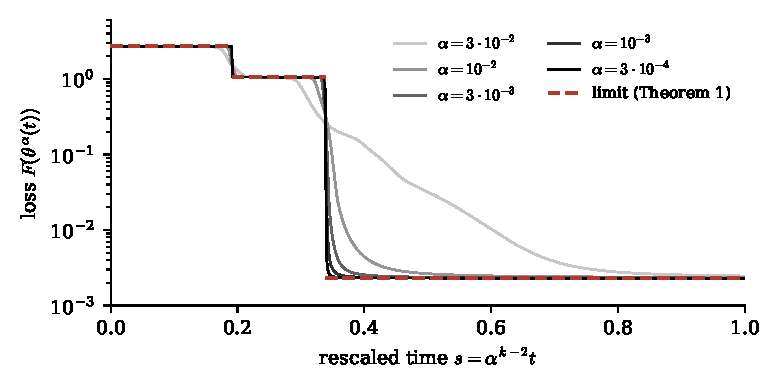
\includegraphics[width=0.85\textwidth]{loss_curves.pdf}
\caption{Loss of gradient flow from $\alpha\xi$ against the rescaled time $s=\alpha^{k-2}t$ (here $k=3$), for decreasing $\alpha$. The dashed line is the limit predicted by Theorem~\ref{thm:main}. The plateau at $0.957$, of duration $5\cdot10^{-4}$, is not visible at this scale.}
\label{fig:loss}
\end{figure}

\begin{thebibliography}{99}\small

\bibitem{BSJ25} I.~Bantzis, J.~B.~Simon, A.~Jacot. Saddle-to-saddle dynamics in deep ReLU networks: low-rank bias in the first saddle escape. International Conference on Learning Representations (ICLR), 2026. arXiv:2505.21722.

\bibitem{JGSHG21} A.~Jacot, F.~Ged, B.~\c{S}im\c{s}ek, C.~Hongler, F.~Gabriel. Saddle-to-saddle dynamics in deep linear networks: small initialization training, symmetry, and sparsity. Preprint, 2021. arXiv:2106.15933.

\bibitem{KH24} A.~Kumar, J.~Haupt. Directional convergence near small initializations and saddles in two-homogeneous neural networks. Transactions on Machine Learning Research, 2024. arXiv:2402.09226.

\bibitem{KH24b} A.~Kumar, J.~Haupt. Early directional convergence in deep homogeneous neural networks for small initializations. Preprint, 2024. arXiv:2403.08121.

\bibitem{KH25} A.~Kumar, J.~Haupt. Towards understanding gradient flow dynamics of homogeneous neural networks beyond the origin. Preprint, 2025. arXiv:2502.15952.

\bibitem{KMC25} D.~Kunin, G.~L.~Marchetti, F.~Chen, D.~Karkada, J.~B.~Simon, M.~R.~DeWeese, S.~Ganguli, N.~Miolane. Alternating gradient flows: a theory of feature learning in two-layer neural networks. NeurIPS, 2025. arXiv:2506.06489.

\bibitem{Loj84} S.~{\L}ojasiewicz. Sur les trajectoires du gradient d'une fonction analytique. Seminari di Geometria 1982--1983, Universit\`a di Bologna, 115--117, 1984.

\bibitem{PF23} S.~Pesme, N.~Flammarion. Saddle-to-saddle dynamics in diagonal linear networks. NeurIPS, 2023. arXiv:2304.00488.

\bibitem{TBLEL26} J.~Town, E.~Boursier, B.~Lewis, M.~Englert, R.~Lazic. Mildly overparameterized ReLU networks on orthogonal data: incremental learning and implicit bias. Preprint, 2026. arXiv:2605.27097.

\end{thebibliography}

\end{document}
